
We will introduce some statistical functions to summarize data. To demonstrate some of these functions, let's first generate some data:

\begin{knitrout}
\definecolor{shadecolor}{rgb}{0.969, 0.969, 0.969}\color{fgcolor}\begin{kframe}
\begin{alltt}
\hlstd{n} \hlkwb{<-} \hlnum{10000}
\hlstd{lambda} \hlkwb{<-} \hlnum{10}
\hlstd{x} \hlkwb{<-} \hlopt{-}\hlkwd{log}\hlstd{(}\hlkwd{runif}\hlstd{(n))}\hlopt{/}\hlstd{lambda}
\end{alltt}
\end{kframe}
\end{knitrout}

Note that in \R, the \code{log} function uses the natural logarithm by default. To use base 10 or base 2, use \code{log10} and \code{log2}, respectively. To specify the base, use the \code{base} argument. For example, try  \code{log(16, base=4)}.

The most commonly used one is the mean (a.k.a. the average), $\overline{x}$:\\
$$\overline{x}=\frac{x_1+\ldots+x_n}{n}\,.$$
Other ways to estimate some sort of `central tendency' of a distribution are:
 \begin{itemize}
 \item The trimmed mean, which is similar to the mean, except that the smallest and largest $p\cdot 100\%$  of the values are excluded from the computation. In our example, if we take $p=0.1$ with the simulated data, only 8,000 data points will be used in the calculation of the trimmed mean; 
 \item The median, which is a number (denoted here by $x_{0.5}$) such that half the data points are greater than $x_{0.5}$ and half are less than or equal to $x_{0.5}$. 
 \end{itemize}

Let's compute the sample's mean, trimmed mean, and median. Notice that  in this example the mean is greater than trimmed mean, which is greater than the median. In general, the mean is not a great estimate of the `center' of a non-symmetric distribution. We say that the mean is more `sensitive to extreme values' than the median.
\begin{knitrout}
\definecolor{shadecolor}{rgb}{0.969, 0.969, 0.969}\color{fgcolor}\begin{kframe}
\begin{alltt}
\hlkwd{mean}\hlstd{(x)}
\end{alltt}
\begin{verbatim}
Output: [1] 0.1007422
\end{verbatim}
\begin{alltt}
\hlkwd{mean}\hlstd{(x,} \hlkwc{trim}\hlstd{=}\hlnum{0.1}\hlstd{)}
\end{alltt}
\begin{verbatim}
Output: [1] 0.08366724
\end{verbatim}
\begin{alltt}
\hlkwd{median}\hlstd{(x)}
\end{alltt}
\begin{verbatim}
Output: [1] 0.07046186
\end{verbatim}
\end{kframe}
\end{knitrout}

The formula we used to generate the data is the probability function of the exponential distribution, with rate parameter $\lambda=10$. We denote it by $X\sim exp(\lambda)$. The exponential distribution is often used to model random waiting times, like the time between incoming text messages. We would usually generate it by using the \code{rexp()} function in \R.
Mathematical analysis of the distribution leads to the fact that the expected value of an exponential random variable with rate $\lambda$, is $1/\lambda$. We see that the theoretical expected value of our example is 0.1, and the sample mean is very close to 0.1. This is no coincidence - we will discuss it in  later chapter.


The distribution of \texttt{x} is shown below as a \textit{box-and-whisker plot} (or simply, boxplot). This is a very simple representation of numeric data, which is constructed by summarizing the data using a few numeric characteristics. The boxplot below is drawn horizontally, and the vertical grey line inside the box is the median. Similar to the median, we find the first quartile -- a point, $x_{0.25}$, such that 25\% of the values are less than $x_{0.25}$ and 75\% are greater than $x_{25}$; and the third quartile -- a point, $x_{0.75}$, such that 75\% of the values are less than $x_{0.75}$ and 25\% are greater than $x_{0.75}$. The first and third quartiles are the vertical edges of the box, also called the lower and upper hinges. So, the box represents 50\% of the data. The range between the first and third quartiles is called the \textit{Inter-Quartile Range}, or IQR, which is sometimes used to estimate the dispersion or spread of the data.
The `whiskers', which are the dashed grey lines, are constructed by adding 1.5$\cdot$IQR to each side of the box. If the result is smaller than the minimum value (or greater than the maximum), then the whisker only extends to the minimum (maximum). Points within the range between the two whiskers are not plotted individually, since their distribution is summarized succinctly by the box-and-whiskers plot. Points outside the range between the two whiskers are considered `outliers', or extreme values, and are shown explicitly. 

The plot was generated with the following code. Try it, and try changing some of the parameters to understand their role. We will cover the topic of visualization in a different chapter.

\begin{knitrout}
\definecolor{shadecolor}{rgb}{0.969, 0.969, 0.969}\color{fgcolor}\begin{kframe}
\begin{alltt}
\hlkwd{boxplot}\hlstd{(x,} \hlkwc{cex}\hlstd{=}\hlnum{0.5}\hlstd{,} \hlkwc{col}\hlstd{=}\hlnum{4}\hlstd{,}\hlkwc{border} \hlstd{=} \hlstr{"grey66"}\hlstd{,} \hlkwc{horizontal} \hlstd{= T,} \hlkwc{axes}\hlstd{=F,} \hlkwc{at}\hlstd{=}\hlnum{0.25}\hlstd{)}
\hlkwd{axis}\hlstd{(}\hlnum{1}\hlstd{,} \hlkwc{pos} \hlstd{=} \hlnum{0}\hlstd{)}
\hlkwd{points}\hlstd{(}\hlkwd{mean}\hlstd{(x),}\hlnum{0.25}\hlstd{,}\hlkwc{col}\hlstd{=}\hlnum{2}\hlstd{,} \hlkwc{pch}\hlstd{=}\hlnum{19}\hlstd{,} \hlkwc{cex}\hlstd{=}\hlnum{0.7}\hlstd{)}
\hlkwd{points}\hlstd{(}\hlkwd{mean}\hlstd{(x,} \hlkwc{trim}\hlstd{=}\hlnum{0.1}\hlstd{),}\hlnum{0.25}\hlstd{,} \hlkwc{col}\hlstd{=}\hlstr{"brown"}\hlstd{,} \hlkwc{pch}\hlstd{=}\hlnum{18}\hlstd{)}
\end{alltt}
\end{kframe}\begin{figure}

{\centering 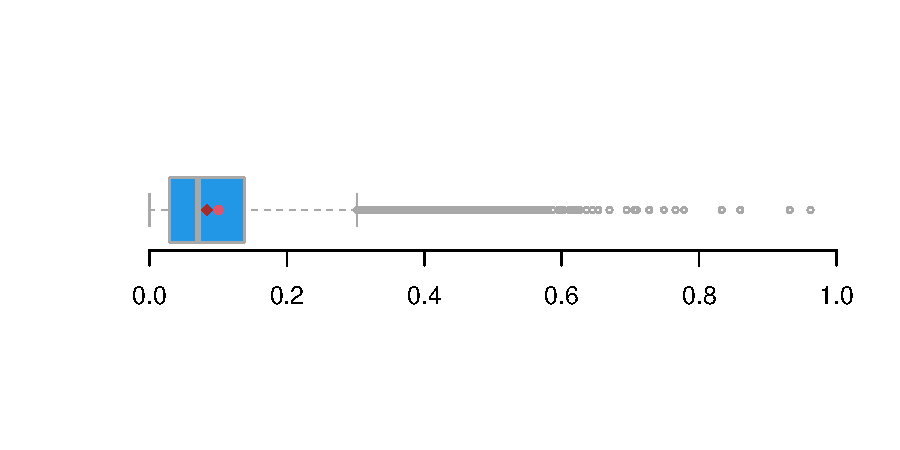
\includegraphics[width=\maxwidth]{figure/intro-boxplot-rexp-1} 

}

\caption[A boxplot]{A boxplot.}\label{fig:intro-boxplot-rexp}
\end{figure}

\end{knitrout}


A boxplot does not include the mean, or the trimmed mean, but we have added them here as a red circle and brown diamond, respectively, in order to show that they are different than the mean. The median is smaller than the mean in this case, so we say that the distribution is skewed to the left. The median does not depend on the scale of the data. It simply represents where half the data lies. 

A more detailed summary of a sample can be obtained by calculating its quantiles. In the boxplot, only three quantiles (also called percentiles) are shown. We can show the quintiles (20, 40, 60, 80 percentiles), or deciles (10, 20,\ldots, 90 percentiles) by using the \code{quantile()} function.

\begin{knitrout}
\definecolor{shadecolor}{rgb}{0.969, 0.969, 0.969}\color{fgcolor}\begin{kframe}
\begin{alltt}
\hlkwd{hist}\hlstd{(x,} \hlkwc{breaks}\hlstd{=}\hlnum{50}\hlstd{,} \hlkwc{border}\hlstd{=}\hlstr{"white"}\hlstd{,} \hlkwc{col}\hlstd{=}\hlstr{"lightblue"}\hlstd{,} \hlkwc{freq}\hlstd{=}\hlnum{FALSE}\hlstd{,} \hlkwc{xlim}\hlstd{=}\hlkwd{c}\hlstd{(}\hlnum{0}\hlstd{,}\hlnum{0.6}\hlstd{))}
\hlstd{deciles} \hlkwb{<-} \hlkwd{quantile}\hlstd{(x,} \hlkwc{probs}\hlstd{=}\hlkwd{seq}\hlstd{(}\hlnum{0.1}\hlstd{,}\hlnum{0.9}\hlstd{,}\hlkwc{by}\hlstd{=}\hlnum{0.1}\hlstd{))}
\hlkwd{abline}\hlstd{(}\hlkwc{v}\hlstd{=deciles,} \hlkwc{lty}\hlstd{=}\hlnum{2}\hlstd{,} \hlkwc{col}\hlstd{=}\hlstr{"purple"}\hlstd{,} \hlkwc{lwd}\hlstd{=}\hlnum{2}\hlstd{)}
\hlkwd{text}\hlstd{(deciles,} \hlkwd{dexp}\hlstd{(deciles,} \hlnum{10}\hlstd{),} \hlkwd{paste0}\hlstd{(}\hlkwd{seq}\hlstd{(}\hlnum{10}\hlstd{,}\hlnum{90}\hlstd{,}\hlkwc{by}\hlstd{=}\hlnum{10}\hlstd{),}\hlstr{"%"}\hlstd{),} \hlkwc{cex}\hlstd{=}\hlnum{0.7}\hlstd{,} \hlkwc{col}\hlstd{=}\hlstr{"orange"}\hlstd{)}
\end{alltt}
\end{kframe}\begin{figure}

{\centering 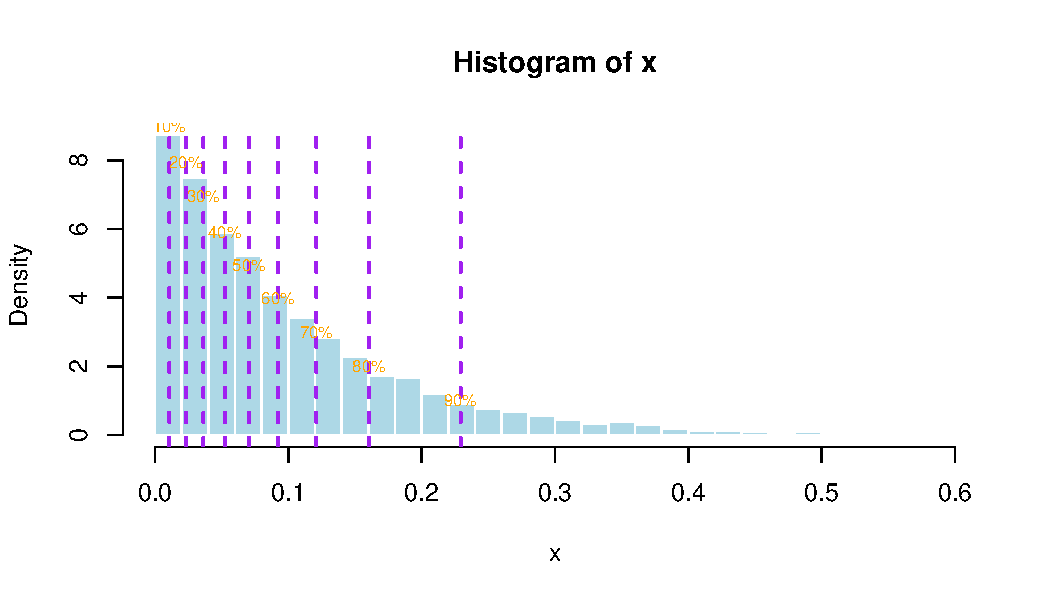
\includegraphics[width=\maxwidth]{figure/intro-quantile-rexp-1} 

}

\caption[A histogram of a sample from an exponential distribution, with the 10, 20, 30,..]{A histogram of a sample from an exponential distribution, with the 10, 20, 30,... percentiles}\label{fig:intro-quantile-rexp}
\end{figure}

\end{knitrout}


In addition to sample statistics which summarize some notion of the center of the distribution, we are often interested in estimating the dispersion of the data. The most commonly used measures of dispersion are the variance, and its square root - the standard deviation. The variance is defined as follows

$$Var(X)=\frac{(x_1-\mu)^2+\ldots+(x_n-\mu)^2}{n}$$
 where $\mu$ is the mean of the distribution of $X$. In words, the variance is the average squared deviation from the mean.
Notice that in \R the variance is computed with n-1 in the denominator (with n-1 we get an `unbiased estimator' for the true variance).

The corresponding functions in \R are \code{var()} and \code{sd()}. In the following code we also demonstrate the \code{IQR()} function.
\begin{knitrout}
\definecolor{shadecolor}{rgb}{0.969, 0.969, 0.969}\color{fgcolor}\begin{kframe}
\begin{alltt}
\hlkwd{var}\hlstd{(x)}
\end{alltt}
\begin{verbatim}
Output: [1] 0.01010772
\end{verbatim}
\begin{alltt}
\hlkwd{sd}\hlstd{(x)} \hlcom{# note that sd(x) is sqrt(sd(x))}
\end{alltt}
\begin{verbatim}
Output: [1] 0.1005371
\end{verbatim}
\begin{alltt}
\hlkwd{IQR}\hlstd{(x)}
\end{alltt}
\begin{verbatim}
Output: [1] 0.1091089
\end{verbatim}
\end{kframe}
\end{knitrout}

We will see in subsequent chapters that the normal distribution plays a major role in statistics. It is defined by a probability density function, with two parameters -- $\mu$ and $\sigma^2$:
$$\phi(x; \mu,\sigma^2)=\frac{1}{\sqrt{2\pi\sigma^2}}\exp\left[-\frac{(x-\mu)^2}{2\sigma^2}\right]\,.$$
It is symmetric, `bell-shaped', and centered around the mean, $\mu$, as shown in the following plot. The blue histogram is generated by the \code{rnorm()} function, using $\mu=2.5$ and $\sigma^2=0.25$. The orange curve shows the function $\phi$, by using the \code{dnorm()} function (to obtain the density of $x$).
\begin{knitrout}
\definecolor{shadecolor}{rgb}{0.969, 0.969, 0.969}\color{fgcolor}\begin{kframe}
\begin{alltt}
\hlstd{x} \hlkwb{<-} \hlkwd{rnorm}\hlstd{(}\hlnum{10000}\hlstd{,} \hlkwc{mean}\hlstd{=}\hlnum{2.5}\hlstd{,} \hlkwc{sd}\hlstd{=}\hlnum{0.5}\hlstd{)}
\hlkwd{hist}\hlstd{(x,} \hlkwc{breaks}\hlstd{=}\hlnum{30}\hlstd{,} \hlkwc{border}\hlstd{=}\hlstr{"white"}\hlstd{,} \hlkwc{col}\hlstd{=}\hlstr{"navyblue"}\hlstd{,} \hlkwc{freq}\hlstd{=}\hlnum{FALSE}\hlstd{)}
\hlstd{xs} \hlkwb{<-} \hlkwd{seq} \hlstd{(}\hlnum{0}\hlstd{,}\hlnum{5}\hlstd{,} \hlkwc{length}\hlstd{=}\hlnum{500}\hlstd{)}
\hlkwd{lines}\hlstd{(xs,} \hlkwd{dnorm}\hlstd{(xs,}\hlnum{2.5}\hlstd{,} \hlnum{0.5}\hlstd{),} \hlkwc{col}\hlstd{=}\hlstr{"orange"}\hlstd{,} \hlkwc{lwd}\hlstd{=}\hlnum{3}\hlstd{)}
\end{alltt}
\end{kframe}\begin{figure}

{\centering 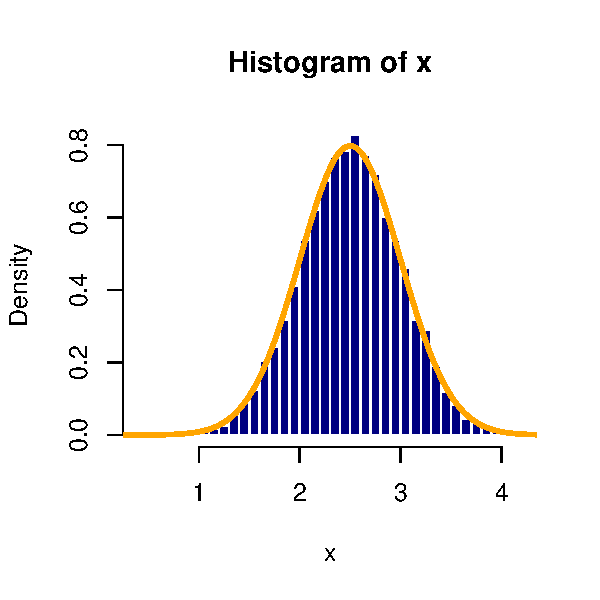
\includegraphics[width=\maxwidth]{figure/intro-rnorm1-1} 

}

\caption[A histogram of a sample from an normal distribution, with mean=2.5 and variance=0.25]{A histogram of a sample from an normal distribution, with mean=2.5 and variance=0.25}\label{fig:intro-rnorm1}
\end{figure}

\end{knitrout}

We can obtained more detailed summaries about the sample, by using the functions \code{summary()} and \code{describe()} (the latter is from the psych package, and provides more details.)

\begin{knitrout}
\definecolor{shadecolor}{rgb}{0.969, 0.969, 0.969}\color{fgcolor}\begin{kframe}
\begin{alltt}
\hlkwd{print}\hlstd{(}\hlkwd{summary}\hlstd{(x))}
\end{alltt}
\begin{verbatim}
Output:    Min. 1st Qu.  Median    Mean 3rd Qu.    Max. 
Output:  0.4667  2.1731  2.5068  2.5043  2.8377  4.1818
\end{verbatim}
\begin{alltt}
\hlkwd{print}\hlstd{(psych}\hlopt{::}\hlkwd{describe}\hlstd{(x))}
\end{alltt}
\begin{verbatim}
Output:    vars     n mean  sd median trimmed  mad  min  max range  skew kurtosis se
Output: X1    1 10000  2.5 0.5   2.51    2.51 0.49 0.47 4.18  3.72 -0.03     0.05  0
\end{verbatim}
\end{kframe}
\end{knitrout}

\code{summary()}  gives the minimum, maximum, the 25th, 50th, and 75th percentiles, as well as the mean of the sample. \code{psych::describe()} also gives the sample size, the standard deviation, the trimmed mean, the mean absolute deviation (mad), the range (maximum minus minimum), the skewness, and the kurtosis \hb{will we use the kurtosis later? If so, we should add a ref.}.

We conclude this chapter with some functions which can be used to summarize discrete (categorical) data, where the mean, variance, quantiles, etc. are not applicable. We will revisit the topic of summarizing data in the chapter on \hb{visualization}.

To simulate categorical data we can use the \code{rmultinom()} function, which simulates putting $N$ objects in $K$ bins with given probabilities. Another possibility is to use \code{cut()} function which divides a range of number into discrete ranges and creates discrete categories in a factor variable.
For example, suppose there is a town with three hotels (Motel 6, Best Western,  and Hilton) with 400, 300, and 300 rooms, and one auto rental company with only two makes of cars (700 Honda, and 300 Teslas). In the following code we simulate the allocation of 100 visitors to hotels and cars. We use the \code{table()} function to show the counts by hotel, by car, and by both. 

\begin{knitrout}
\definecolor{shadecolor}{rgb}{0.969, 0.969, 0.969}\color{fgcolor}\begin{kframe}
\begin{alltt}
\hlstd{hotelrooms} \hlkwb{<-} \hlkwd{cut}\hlstd{(}\hlkwd{runif}\hlstd{(}\hlnum{100}\hlstd{),}\hlkwc{breaks} \hlstd{=} \hlkwd{c}\hlstd{(}\hlnum{0}\hlstd{,}\hlnum{0.4}\hlstd{,}\hlnum{0.7}\hlstd{,}\hlnum{1}\hlstd{),} \hlkwc{include.lowest} \hlstd{=} \hlnum{TRUE}\hlstd{)}
\hlkwd{levels}\hlstd{(hotelrooms)} \hlkwb{<-} \hlkwd{c}\hlstd{(}\hlstr{"Motel 6"}\hlstd{,} \hlstr{"Best Western"}\hlstd{,} \hlstr{"Hilton"}\hlstd{)}
\hlstd{autorental} \hlkwb{<-} \hlkwd{cut}\hlstd{(}\hlkwd{runif}\hlstd{(}\hlnum{100}\hlstd{),}\hlkwc{breaks} \hlstd{=} \hlkwd{c}\hlstd{(}\hlnum{0}\hlstd{,}\hlnum{0.7}\hlstd{,}\hlnum{1}\hlstd{),} \hlkwc{include.lowest} \hlstd{=} \hlnum{TRUE}\hlstd{)}
\hlkwd{levels}\hlstd{(autorental)} \hlkwb{<-} \hlkwd{c}\hlstd{(}\hlstr{"Honda"}\hlstd{,} \hlstr{"Tesla"}\hlstd{)}
\hlstd{(hoteltbl} \hlkwb{<-} \hlkwd{table}\hlstd{(hotelrooms))}
\end{alltt}
\begin{verbatim}
Output: hotelrooms
Output:      Motel 6 Best Western       Hilton 
Output:           45           27           28
\end{verbatim}
\begin{alltt}
\hlstd{(autotbl} \hlkwb{<-} \hlkwd{table}\hlstd{(autorental))}
\end{alltt}
\begin{verbatim}
Output: autorental
Output: Honda Tesla 
Output:    69    31
\end{verbatim}
\begin{alltt}
\hlkwd{table}\hlstd{(hotelrooms, autorental)}
\end{alltt}
\begin{verbatim}
Output:               autorental
Output: hotelrooms     Honda Tesla
Output:   Motel 6         27    18
Output:   Best Western    21     6
Output:   Hilton          21     7
\end{verbatim}
\end{kframe}
\end{knitrout}

We can use the \code{max()} and \code{which.max()} functions to find the mode of the data (the most frequent value).

\begin{knitrout}
\definecolor{shadecolor}{rgb}{0.969, 0.969, 0.969}\color{fgcolor}\begin{kframe}
\begin{alltt}
\hlkwd{cat}\hlstd{(}\hlkwd{levels}\hlstd{(hotelrooms)[}\hlkwd{which.max}\hlstd{(hoteltbl)],}\hlstr{":"}\hlstd{,} \hlkwd{max}\hlstd{(hoteltbl),}\hlstr{"\textbackslash{}n"}\hlstd{)}
\end{alltt}
\begin{verbatim}
Output: Motel 6 : 45
\end{verbatim}
\begin{alltt}
\hlkwd{cat}\hlstd{(}\hlkwd{levels}\hlstd{(autorental)[}\hlkwd{which.max}\hlstd{(autotbl)],}\hlstr{":"}\hlstd{,} \hlkwd{max}\hlstd{(autotbl),}\hlstr{"\textbackslash{}n"}\hlstd{)}
\end{alltt}
\begin{verbatim}
Output: Honda : 69
\end{verbatim}
\end{kframe}
\end{knitrout}

%matrices
% in a chapter on visualization:
%.  more distributions - Poisson, beta, gamma, lognormal
%.  density plot
%.  ecdf
%.  Q-Q plot
%.  scatterplot
